% !TEX root = macfp_2017_gasphase.tex

\subsection{Case 1: Turbulent Buoyant Plumes} \label{sec:buoyant_plumes}

\subsubsection{Experiment}

The buoyant plume experiment selected for the first MaCFP workshop is a turbulent non-reacting helium plume studied at a test facility called the Fire Laboratory for the Accreditation of Models by Experimentation (FLAME) facility at Sandia National Laboratories~(Sandia)~\cite{Blanchat:2001,Case1_EXP}. The original goal of the Sandia buoyant plume experiment was to provide comprehensive turbulent flow velocity and species concentration statistics in a configuration that is representative of large-scale pool fires without the complexities of chemical reactions and temperature variations~\cite{Case1_EXP}.  The 1-m diameter source provides a plume in the fully-developed turbulent flow regime.  

The 1-m diameter helium source was surrounded by a 0.51-m wide steel lip, representing the injection plane and elevated 2.45 m above an annular ring which introduced a low-velocity co-flow of ambient air~\cite{Blanchat:2001}. The FLAME facility can be approximated as a 6.1-m cubic chamber covered by a 2.4-m diameter extraction hood. Planar imaging measurements of velocity and species were conducted using Particle Image Velocimetry and Planar Laser Induced Fluorescence, respectively. Laser measurements were recorded at 200~Hz in a window approximately 0.86~m high and 1.2~m wide, and providing an image of the near-field region (starting from the helium injection plane and centered on the plume centerline). The measurement window includes near-field entertainment zones on both sides of the plume; however, it does not include the lateral and vertical far-field. The experimental uncertainty of the measured velocities and turbulent statistics are reported as 20\% and 30\%, respectively. The uncertainty of the measured helium concentration is reported as 18\%. Inlet conditions are uniform to within 5\% or less for the helium flow and within 10\% for the air coflow. The above uncertainties include run-to-run variability. 

For the purpose of MaCFP, tests no. 25, 29, 32 and 36 were selected corresponding to repeat runs with a helium inlet velocity of 0.339 m/s $\pm 1.3$\%, a flow Reynolds number $Re=3194$~$\pm$ $0.6$\%, a flow Richardson number $Ri=69.53$~$\pm 6.5\%$ and a measured puffing frequency of $1.45$ Hz \cite{Case1_EXP}.

\subsubsection{Simulations}

Three groups submitted computational results for Case 1:  IRSN~\cite{Case1_SIM_IRSN}, NIST~\cite{Case1_SIM_NIST} and UGent~\cite{Case1_SIM_UGent}. Some information was also compared with past results published in the literature by Sandia running Fuego~\cite{DesJardin:2004}. IRSN used ISIS version 4.8.0~\cite{ISIS}; NIST used an official release of FDS (version 6.5.3)~\cite{FDS}; UGent used FireFOAM version 1.6~\cite{FireFOAM}.

As discussed in section~\ref{sec:CGD}, the main challenge found in the design of a computational grid for LES simulations of the Sandia helium plume experiment is to provide suitable grid resolution to capture the intermittent boundary layer and ``thermals" that result from unstable buoyant motions (see Figure~\ref{fig:He-Plume-Scales}). This may require millimeter-scale resolution. The computational groups responded to this challenge in different ways: IRSN adopted a 2.5-cm resolution; NIST adopted a 1.5-cm resolution; UGent adopted a stretched grid with 1.23-cm resolution near the helium source. Note that previous work in Ref.~\cite{DesJardin:2004} used both 3- and 5-cm grid resolution. The computational domain in all simulations is much larger than the measurement region (and is 3- or 4-m wide and 4-m high); however, it does not include all details of the full facility. 

Note that there were some variations among computational groups in the treatment of the co-flow: the air co-flow velocity was introduced through an annular ring located below the helium injection plane with a ring-level velocity approximately equal to 0.15-0.18~m/s~\cite{Blanchat:2001}; IRSN did attempt to model the annular ring but did not use the correct geometry and coflow velocity; in contrast, NIST and UGent did not attempt to model the annular ring and assumed instead simplified boundary conditions at the helium injection plane \-- NIST prescribed a small coflow velocity equal to 0.01~m/s (at the injection plane) while UGent used free entrainment conditions. Also, while NIST and UGent assumed an ambient pressure of 80.9~kPa (due to the high elevation of the FLAME facility), IRSN incorrectly assumed an ambient pressure of 101.1 kPa.

\begin{figure}
\centering
(a)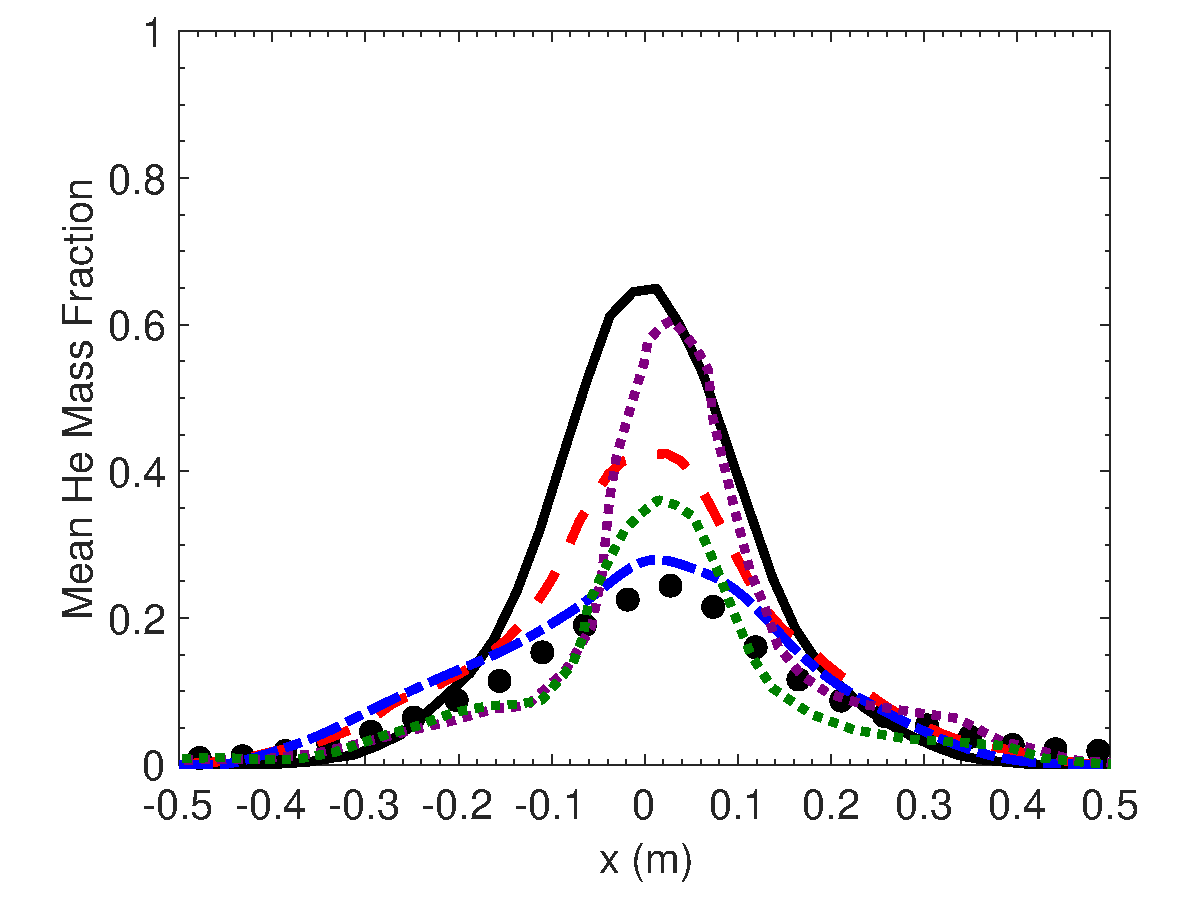
\includegraphics[height=2.2in]{Figures/Case1-Fig1a.pdf}
(b)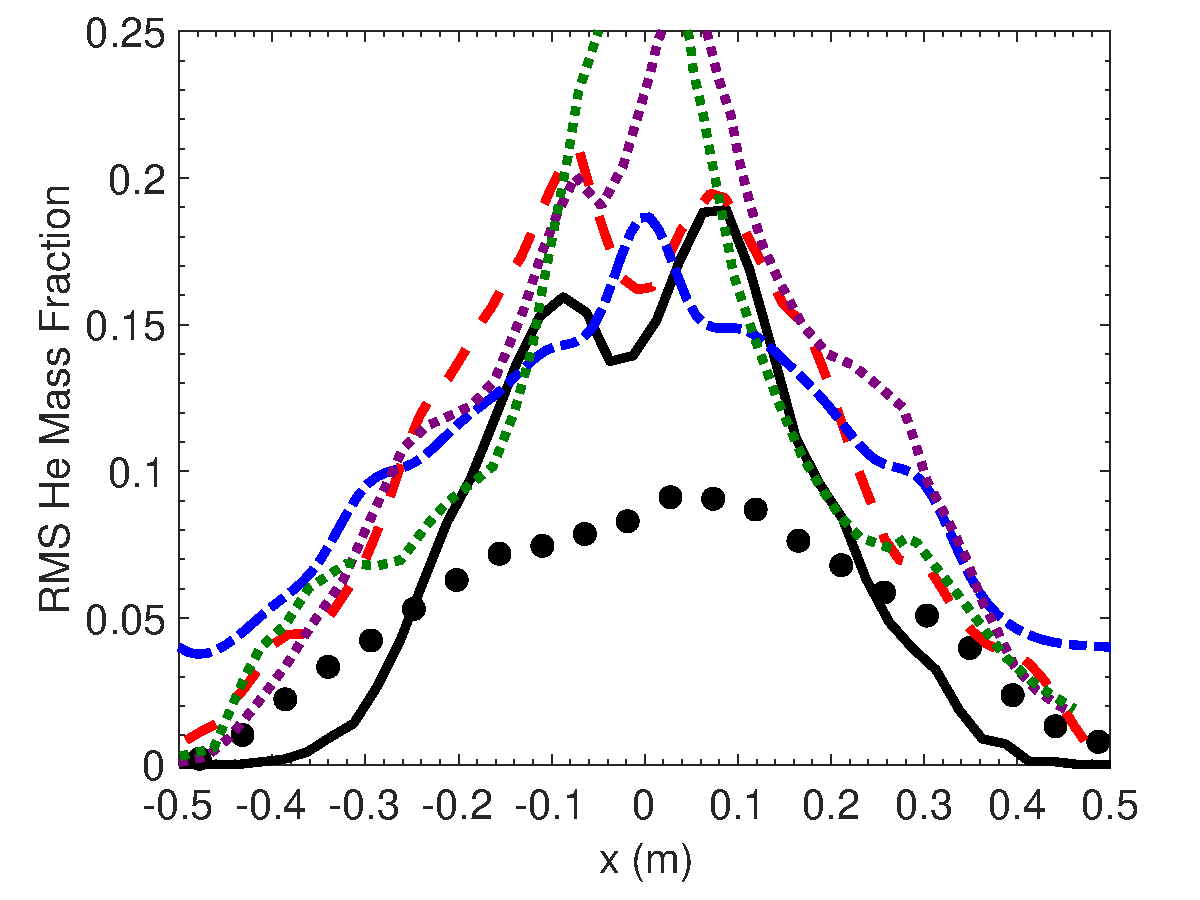
\includegraphics[height=2.2in]{Figures/Case1-Fig1b.pdf}
(c)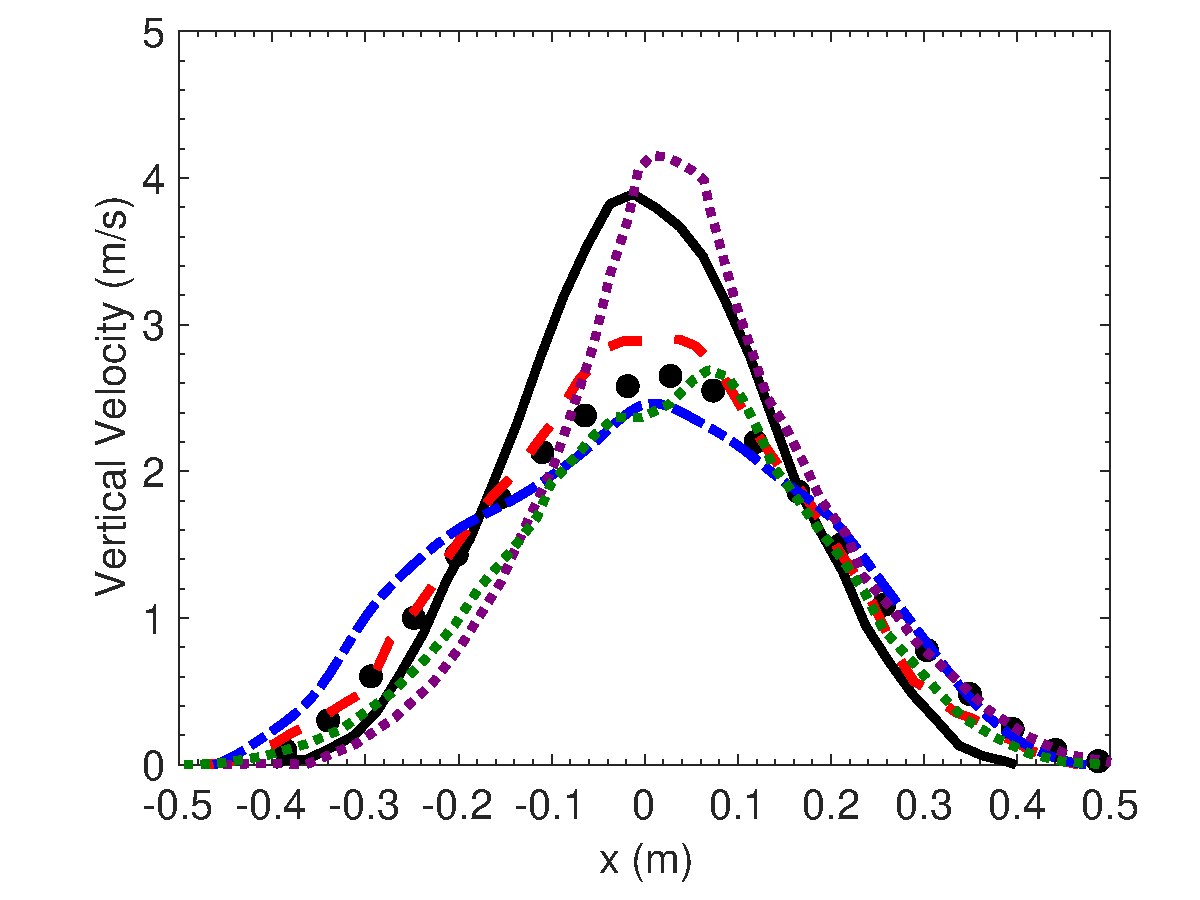
\includegraphics[height=2.2in]{Figures/Case1-Fig1c.pdf}
(d)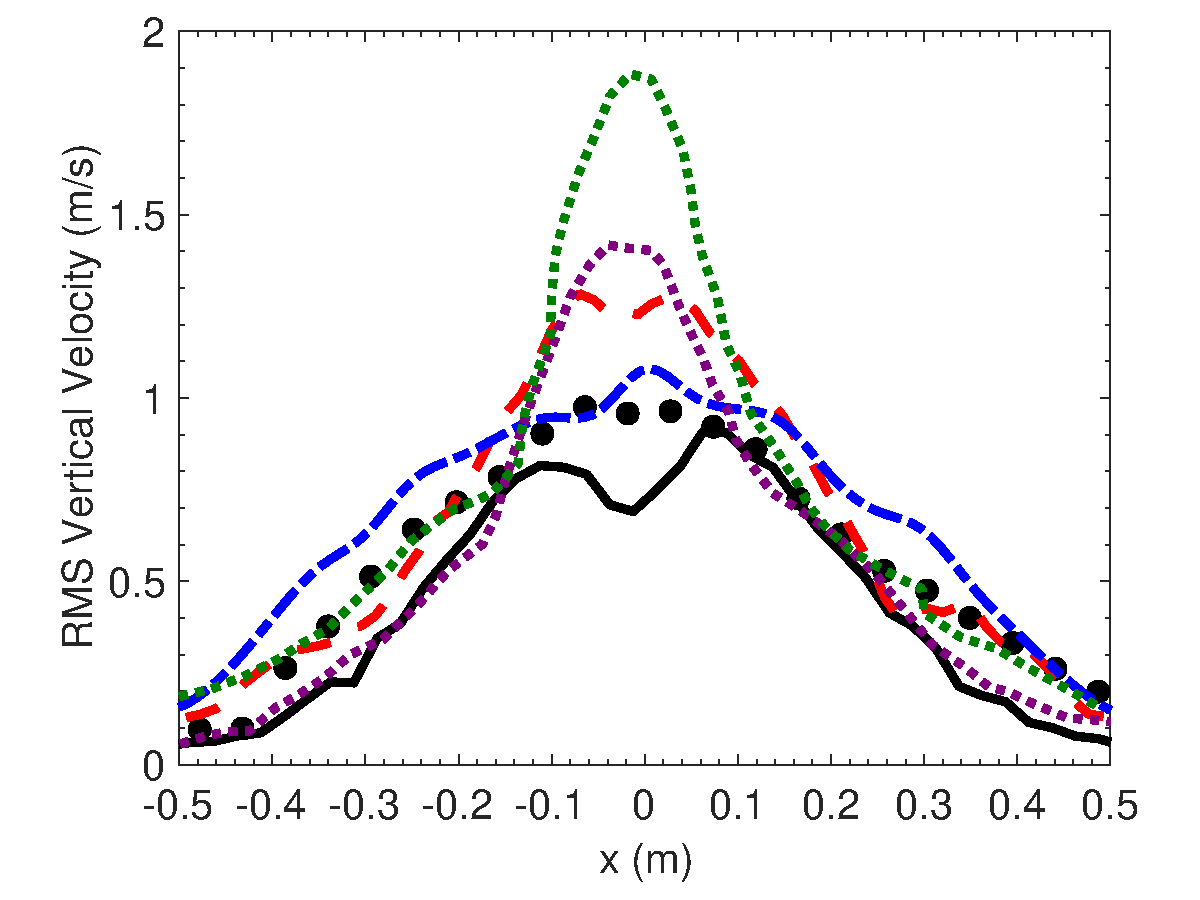
\includegraphics[height=2.2in]{Figures/Case1-Fig1d.pdf}
\caption{Case 1. Radial variations at $z = 0.4$~m of: (a) mean helium mass fraction; (b) {\it rms} helium mass fraction; (c) mean vertical velocity; (d) {\it rms} vertical velocity. Comparison between experimental data (black circles) and numerical results from IRSN (black solid line), NIST (red dashed line), UGent (blue dash-dotted line) and results from Ref.~\cite{DesJardin:2004} (magenta and green dotted lines, corresponding to 5-cm and 3-cm resolution, respectively).}
\label{fig:Case1-Fig1}
\end{figure}

Additional differences in the numerical treatment of the Sandia plume experiment include differences in the choice of physical models (see section~\ref{sec:PM} for details on baseline choices).  IRSN used the baseline configuration of ISIS and NIST used the baseline configuration of FDS. UGent deviated from baseline choices in FireFOAM and used the constant-coefficient Smagorinsky model for subgrid-scale turbulence (additional information can be found in Ref.~\cite{Maragkos:2013}). 

The durations of the simulations and the durations over which numerical results were collected and statistical moments were evaluated varied: IRSN, NIST and UGent chose to run their models for 10~s, 20~s and 30~s, respectively (in Ref.~\cite{DesJardin:2004}, the model was run for 20~s); all groups except IRSN chose to collect numerical results over the last 10~s, corresponding to approximately 14 puffing cycles; IRSN analyzed data over 3~s or approximately 4 puffing cycles (in this case, the results should be analyzed with caution because the statistics may not be converged) .

\subsubsection{Summary}

Figure~\ref{fig:Case1-Fig1} presents a representative sample of comparisons between measured and simulated helium mass fractions and vertical flow velocity. The comparisons generally suggest that accuracy increases with higher levels of grid resolution and that an accurate description of the flow statistics in the near-field region requires a resolution of approximately 1 or 2~cm. Note that this corresponds to 100 or 50 computational cells across the source diameter, a level of resolution that is much higher than the usual requirement of providing a grid spacing that is 10-20 times smaller than the source diameter $D$. In addition, even at this high level of resolution, the magnitude of the fluctuations in helium mass fraction is not captured accurately (see Figure~\ref{fig:Case1-Fig1}(b)). These inconsistent results suggest that the dynamics associated with the presence of both thin boundary layers near the edges of the helium source and small-scale ``thermals" generated by secondary buoyant instabilities play a significant role in determining near-field turbulent mixing properties. Note that the exact impact of the inaccuracies in the near-field on the global flow features of the far-field have not been characterized.

It is worth emphasizing that the experimental database describing the Sandia helium plume experiment is of great value because it contains data on first and second-order statistical moments of flow velocities and helium concentrations measured with high spatial resolution~\cite{Case1_EXP}. There are also some limitations in the database that are worth pointing out for future studies: (1) the Sandia database is limited to the plume near-field, $i.e.$ to low elevations ($z \leq 1.2$~m, $i.e.$ $z < (1.2 \times D$)), and there is a need to provide similar data in the far-field; (2) the Sandia database does not provide much information on the puffing cycle and there is a need to provide phase-averaged data to characterize the coupling between large- and small-scale dynamics.

